\documentclass{beamer}
\usetheme{Warsaw}
\usecolortheme{beaver}
\title[Bias, Variance and Parsimony in Regression Analysis]{Bias, Variance and Parsimony in Regression Analysis\\ECS 256 Winter 2014}
\author[Matloff]{
Christopher Patton, \texttt{cjpatton@ucdavis.edu}\\
Alex Rumbaugh, \texttt{aprumbaugh@ucdavis.edu}\\
Thomas Provan,\texttt{tcprovan@ucdavis.edu}\\
Olga Prilepova, \texttt{prilepova@gmail.com}\\
John Chen, \texttt{jhochen@ucdavis.edu}}
\institute{ECS 256, Winter 2014\\ \Large{UC Davis}}
\date{March 12, 2014}
\begin{document}

\begin{frame}
\titlepage
\end{frame}


\begin{frame}{Introduction}
This is the introduction.
\end{frame}

% Alex's Section -----------------------------------------------------------------

\begin{frame}
    \frametitle{California Housing Data}
	\begin{itemize}
		\item { }
		\item {Derived from 1990 Census}
		\item {Response Variable: median house value}
		\item {Predictor Variables: median income, housing median age, total rooms, total bedrooms, population, households, latitude, and longitude}
	\end{itemize}
\end{frame}

\begin{frame}
    \frametitle{Parsimony}
	\begin{tabular}{ | c | p{3cm} | p{3cm} | c  |}
\hline
Method&Parsimony (k=0.01) & Parsimony (k=0.05) & Significance Testing \\
\hline
Columns\newline Deleted& Total Rooms \newline Total Bedrooms & Total Rooms \newline Total Bedrooms \newline Median Age & None \\
\hline
Adjusted RSquared & 0.6321316 & 0.6218261 & 0.6369649 \\
\hline
\end{tabular}
\end{frame}

\begin{frame}[fragile]
    \frametitle{Regression Coefficients}
\begin{verbatim}
Coefficients:
                 Estimate Std. Error t value Pr(>|t|)    
(Intercept)    -3.594e+06  6.254e+04 -57.468  < 2e-16 ***
Median.Income   4.025e+04  3.351e+02 120.123  < 2e-16 ***
Median.Age      1.156e+03  4.317e+01  26.787  < 2e-16 ***
Total.Rooms    -8.182e+00  7.881e-01 -10.381  < 2e-16 ***
Total.Bedrooms  1.134e+02  6.902e+00  16.432  < 2e-16 ***
Population     -3.854e+01  1.079e+00 -35.716  < 2e-16 ***
Households      4.831e+01  7.515e+00   6.429 1.32e-10 ***
Latitude       -4.258e+04  6.733e+02 -63.240  < 2e-16 ***
Longitude      -4.282e+04  7.130e+02 -60.061  < 2e-16 ***
\end{verbatim}
\end{frame}

\begin{frame}[fragile]
    \frametitle{Latitude \& Longitude}
\begin{verbatim}
	Latitude       -4.258e+04  6.733e+02 -63.240  < 2e-16 ***
	Longitude      -4.282e+04  7.130e+02 -60.061  < 2e-16 ***
\end{verbatim}
\begin{itemize}
\item "Center of Gravity"
\item Avoid Overfitting
\end{itemize}
	
\end{frame}

\begin{frame}[fragile]
    \frametitle{Understanding}
	\begin{verbatim}
Coefficients:
                Estimate Std. Error t value Pr(>|t|)    
(Intercept)   -32165.268   2167.358  -14.84   <2e-16 ***
Median.Income  43094.918    284.263  151.60   <2e-16 ***
Median.Age      2000.544     45.080   44.38   <2e-16 ***
Population       -43.045      1.127  -38.20   <2e-16 ***
Households       152.700      3.344   45.66   <2e-16 ***
\end{verbatim}
\end{frame}

\begin{frame}
	\begin{figure}
 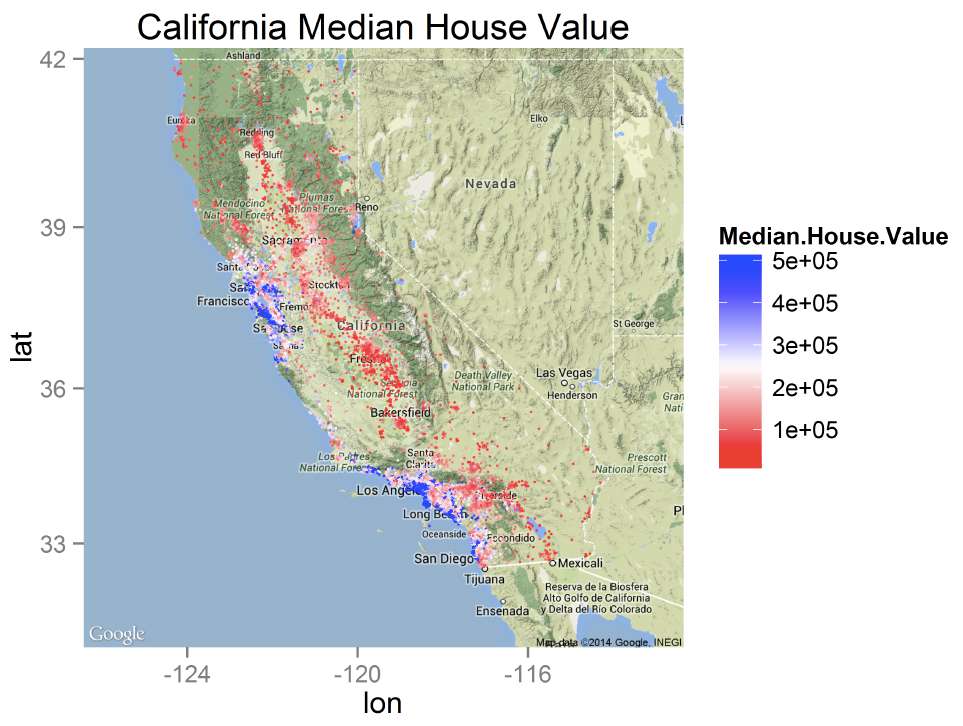
\includegraphics[scale=0.3]{figures/california.png}
\end{figure}
\end{frame}

\begin{frame}
	\begin{figure}
 \includegraphics[scale=0.3]{figures/losangeles.png}
\end{figure}
\end{frame}

\begin{frame}
	\begin{figure}
 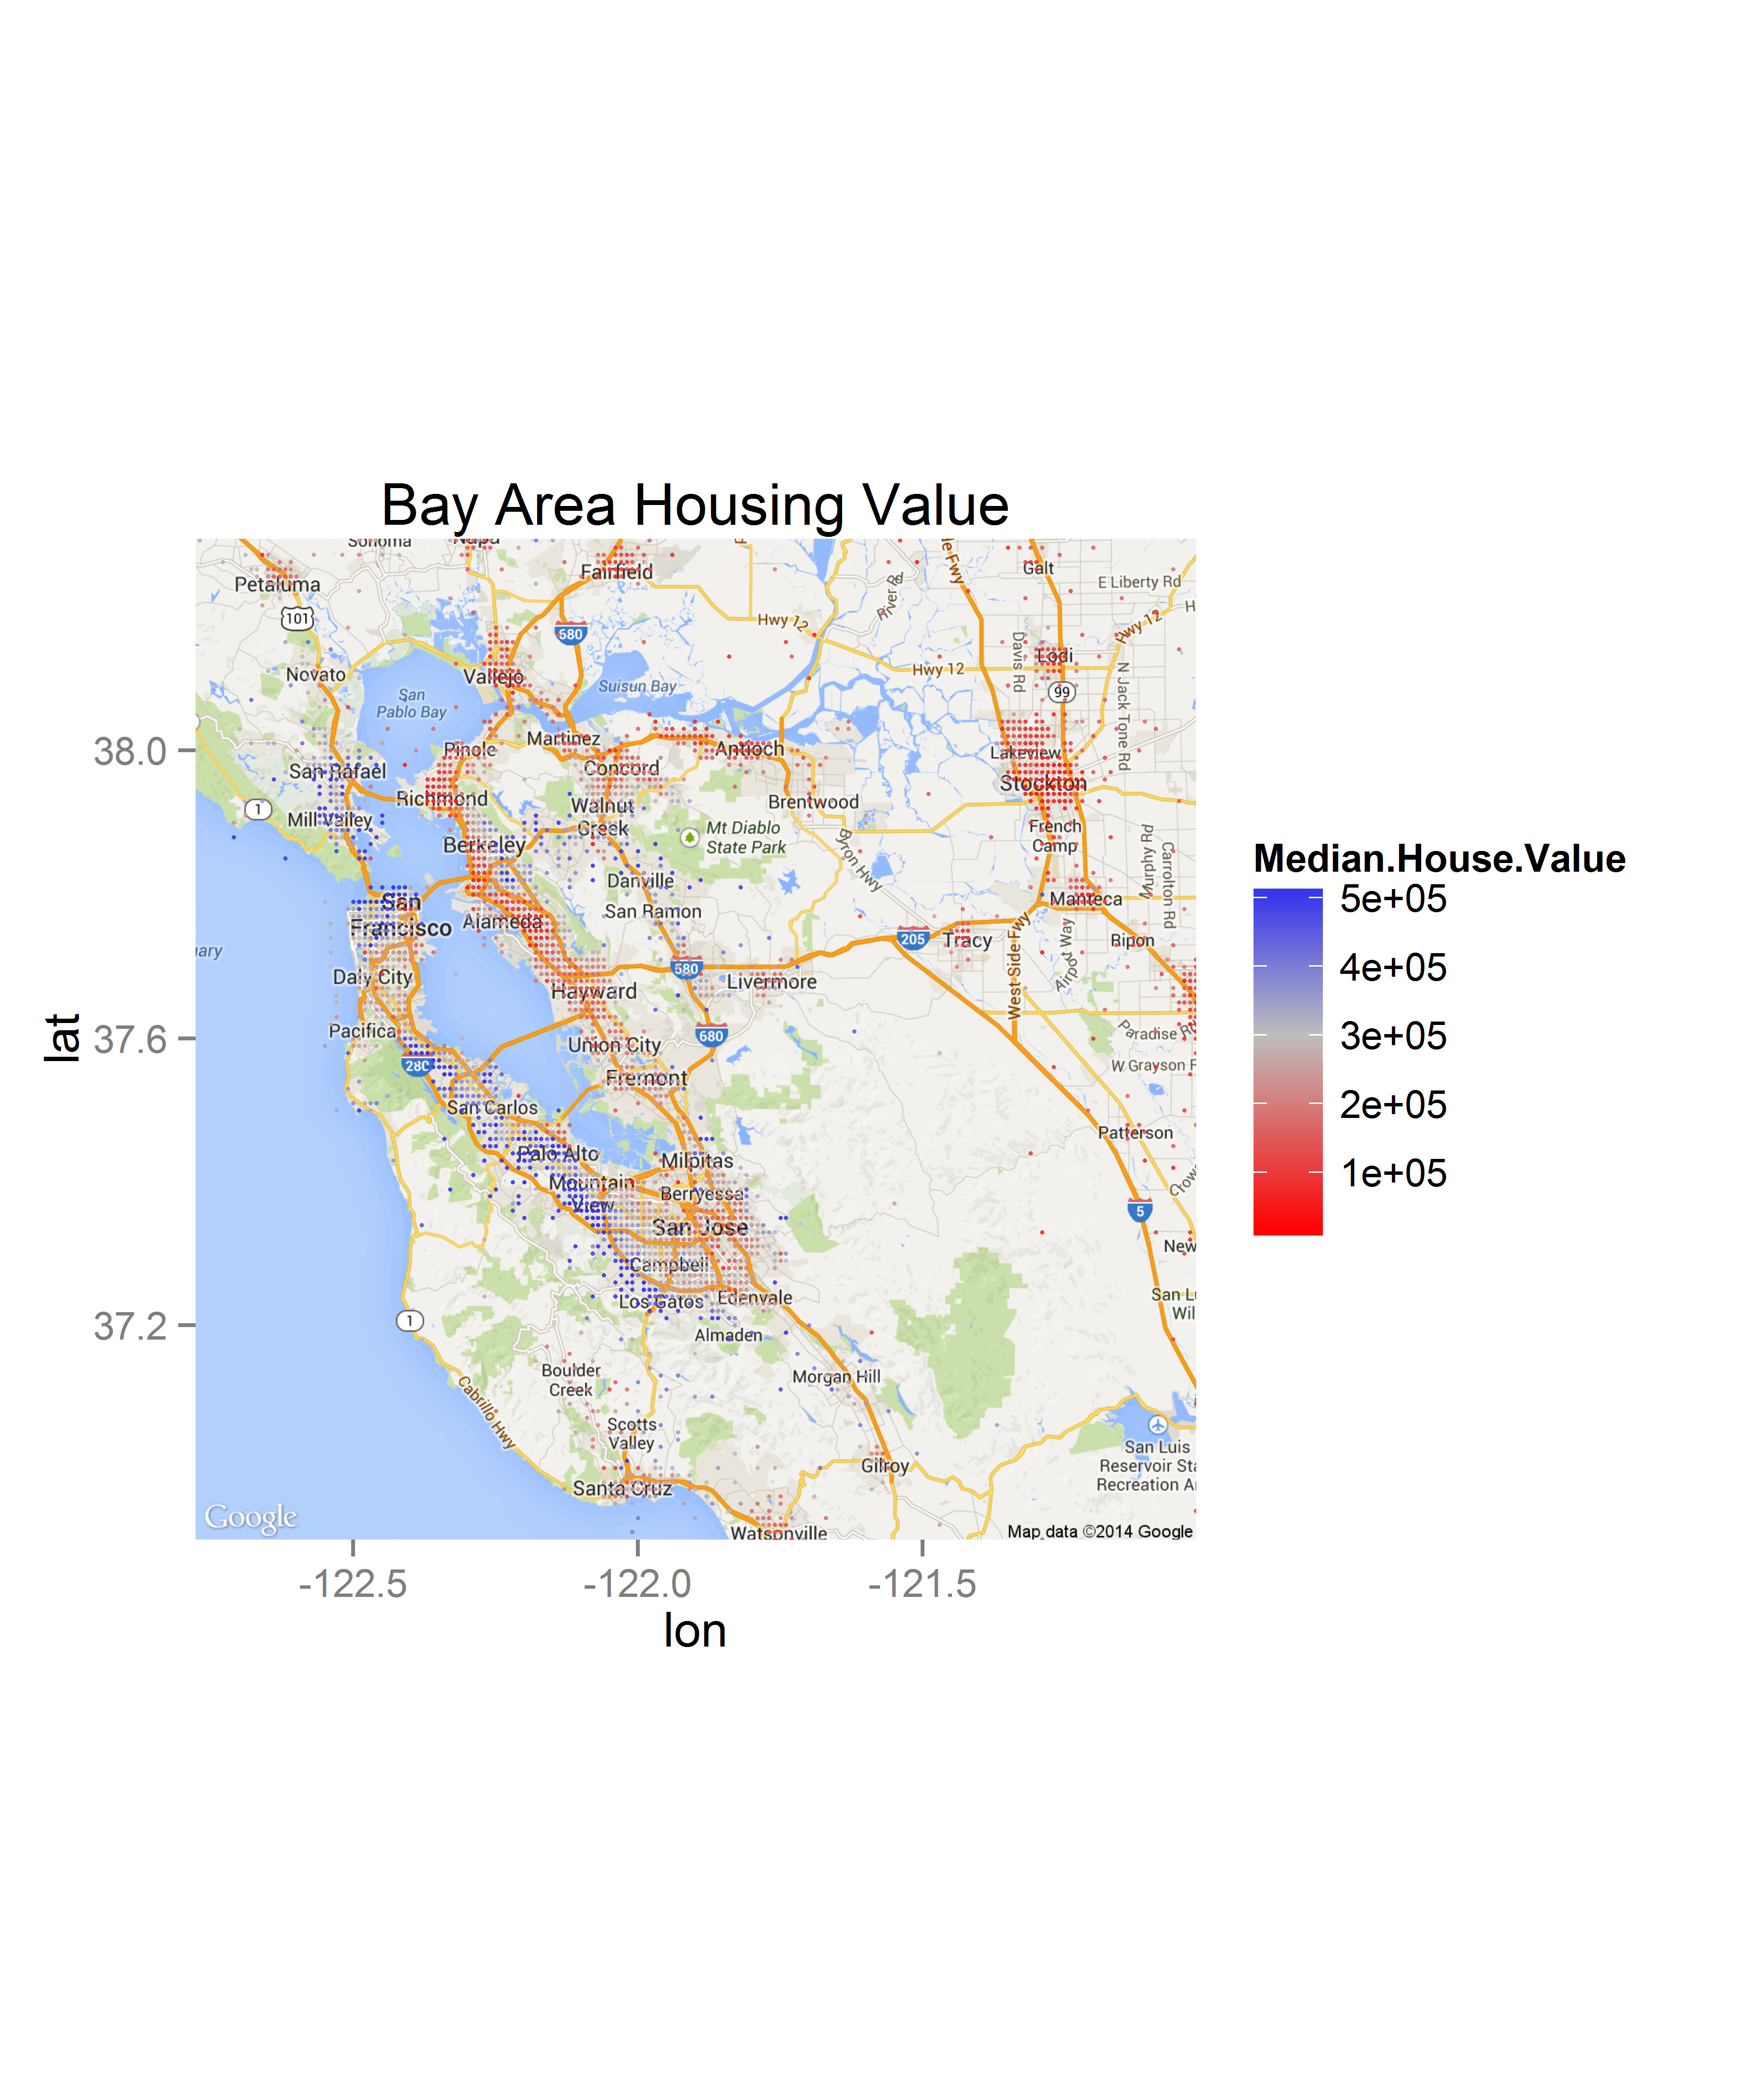
\includegraphics[scale=0.3]{figures/bayarea.png}
\end{figure}
\end{frame}

% End Alex's Section--------------------------------------------------------------

% Olga's Section--------------------------------------------------------------


\begin{frame}
\frametitle{Census Based on 1994}
\end{frame}

\begin{frame}
\frametitle{Age}
\end{frame}

\begin{frame}
\frametitle{}

\begin{figure}
 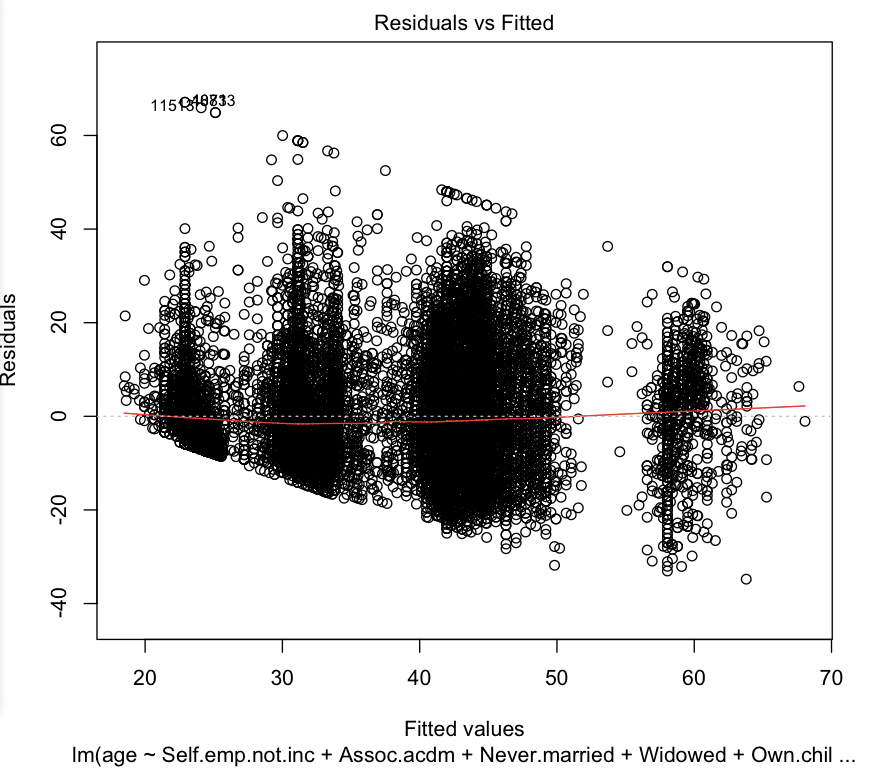
\includegraphics[scale=0.3]{figures/ageResidCensus.png}
 \label{fig:ageResidCensus}
\end{figure}
 
\end{frame}

\begin{frame}
\frametitle{Census Based on 1994}
% Census Sex Coefficients
\end{frame}

\begin{frame}
\frametitle{Census Based on 1994}
% Census Salary Coefficients
\end{frame}

\begin{frame}
%Picture of predicted vs actual age
\begin{figure}
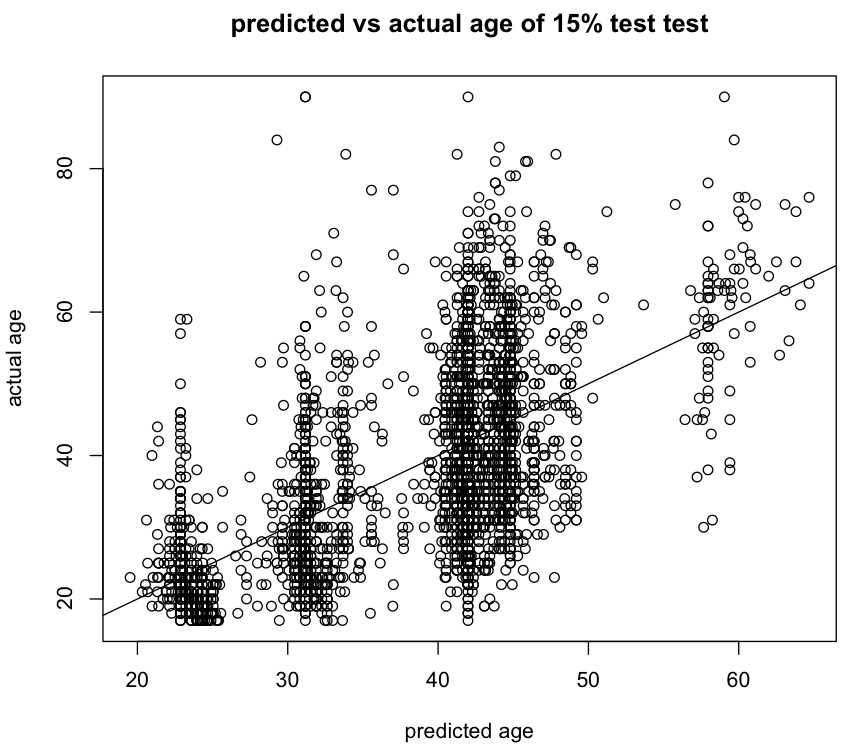
\includegraphics[scale=0.3]{figures/predVsActualCensus.png}
\label{fig:predVsActualCensus}
\end{figure}
\end{frame}

\begin{frame}
%Picture of predicted vs actual age

\begin{figure}
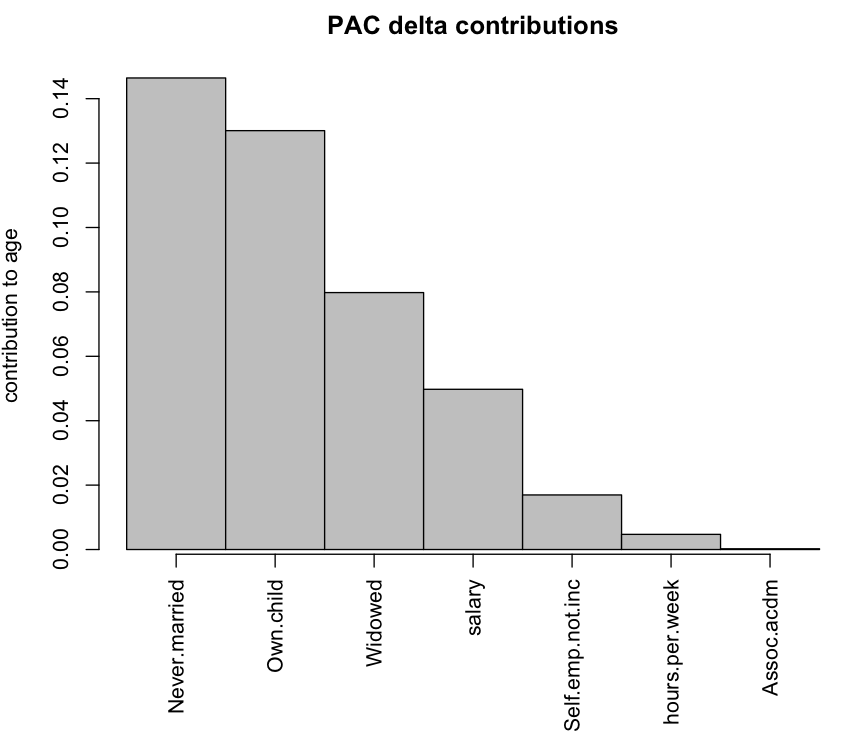
\includegraphics[scale=0.3]{figures/ageContrib.png}
\caption{}
 \label{fig:ageContrib}
\end{figure}

\end{frame}
% End Olga's Section--------------------------------------------------------------

% Begin Chris' Section--------------------------------------------------------------


\begin{frame}
\frametitle{}
%Slide 1
\end{frame}

\begin{frame}
\frametitle{}
%Slide 2
\end{frame}

\begin{frame}
\frametitle{}
%Slide 3
\end{frame}

\begin{frame}
\frametitle{}
%Slide 4
\end{frame}

\begin{frame}
\frametitle{}
%Slide 5
\end{frame}

% End Chris' Section--------------------------------------------------------------
% Thomas' Section--------------------------------------------------------------


\begin{frame}
\frametitle{}
%Slide 1
\end{frame}

\begin{frame}
\frametitle{}
%Slide 2
\end{frame}

\begin{frame}
\frametitle{}
%Slide 3
\end{frame}

\begin{frame}
\frametitle{}
%Slide 4
\end{frame}

\begin{frame}
\frametitle{}
%Slide 5
\end{frame}
% End Thomas' Section--------------------------------------------------------------
% John's Section--------------------------------------------------------------


\begin{frame}
\frametitle{}
%Slide 1
\end{frame}

\begin{frame}
\frametitle{}
%Slide 2
\end{frame}

\begin{frame}
\frametitle{}
%Slide 3
\end{frame}

\begin{frame}
\frametitle{}
%Slide 4
\end{frame}

\begin{frame}
\frametitle{}
%Slide 5
\end{frame}
% End John's Section--------------------------------------------------------------
\end{document}